% Part: history
% Chapter: set-theory
% Section: limits

\documentclass[../../../include/open-logic-section]{subfiles}

\begin{document}
	
\olfileid{his}{set}{limits}	

\olsection{Rigorous Definition of Limits}
	
These days, the standard solution to the foregoing problem is to get
rid of the infinitesimals. Here is how. 

We saw that, as $\beta$ gets smaller, we get better approximations of
the gradient. Indeed, as $\beta$ gets arbitrarily close to $0$, the
value of $f'(c)$ ``tends without limit'' to the gradient we want. So,
instead of considering what happens \emph{at} $\beta = 0$, we need
only consider the \emph{trend} of $f'(c)$ as $\beta$ approaches $0$. 

Put like this, the general challenge is to make sense of claims of
this shape:
\begin{center}
As $x$ approaches $c$, $g(x)$ tends without limit to $\ell$. 
\end{center}
which we can write more compactly as follows:
\[
\lim_{x \rightarrow c}g(x) = \ell.
\]
In the 19th century, building upon earlier work by Cauchy, Weierstrass
offered a perfectly rigorous definition of this expression. The idea
is indeed that we can make $g(x)$ as close as we like to~$\ell$, by
making $x$ suitably close to~$c$. More precisely, we stipulate that
$\lim_{x \rightarrow c} g(x) = \ell$ will mean:
\[
(\exists\ell \in \Real)(\forall\epsilon > 0)(\exists \delta > 0)\forall x \left(0 < |x - c| < \delta \lif |g(x) - \ell| < \epsilon \right).
\]
Here $\ell$ is unique. That is, if both $\ell_1 \in \Real$ and
$\ell_2 \in \Real$ witness the above sentence, it must be the case
that $\ell_1=\ell_2$. We say that the limit of a function is unique.

\begin{prob}
	Prove that the limit of a function is unique.
\end{prob}

The vertical bars here indicate absolute magnitude. That is, $|x| = x$
when $x \geq 0$, and $|x| =-x$ when $x < 0$; you can depict
\emph{that} function as follows:
\begin{center}
	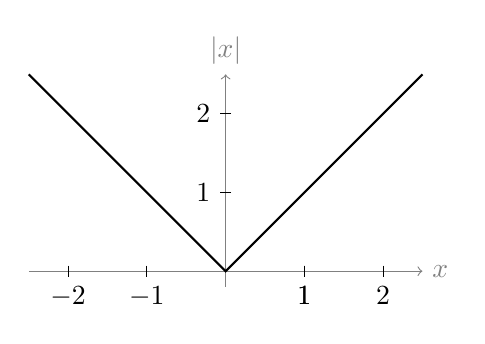
\begin{tikzpicture}[scale=1]
	\draw[->, gray] (-2.5,0) -- (2.5,0) node[right] {$x$};
	\draw[->, gray] (0,-.2) -- (0,2.5) node[above] {$|x|$};
	
	\foreach \x/\xtext in {-2/-2, -1,1, 1/1, 2/2}
	\draw[shift={(\x,0)}] (0pt,2pt) -- (0pt,-2pt) node[below] {{$\xtext$}};
	
	\foreach \y/\ytext in {1/1, 2/2}
	\draw[shift={(0,\y)}] (2pt,0pt) -- (-2pt,0pt) node[left] {{$\ytext$}};
	
	\draw[thick] (-2.5, 2.5)--(0,0)--(2.5, 2.5);
	\end{tikzpicture}
\end{center}
So the definition says roughly this: you can make your ``error'' less
than $\epsilon$ (i.e., $|g(x) - \ell| < \epsilon$) by choosing
arguments which are no more than $\delta$ away from~$c$ (i.e., $|x -
c| < \delta$). 

Having defined the notion of a limit, we can use it to avoid
infinitesimals altogether, stipulating that the gradient of $f$ at $c$
is given by:
\[
	{f}'(c) = \lim_{x \rightarrow 0}\left(\frac{f(c +x) - f(c)}{x}\right) \text{ where a limit exists}.
\]
It is important, though, to realise why our definition needs the
caveat ``where a limit exists''. To take a simple example, consider
$f(x) = |x|$, whose graph we just saw. Evidently, $f'(0)$ is
ill-defined: if we approach $0$ ``from the right'', the gradient is
always $1$; if we approach $0$ ``from the left'', the gradient is
always $-1$; so the limit is undefined. As such, we might add that a
function~$f$ is \emph{differentiable} at~$x$ iff such a limit exists.

We have seen how to handle differentiation using the notion of a
\emph{limit}. We can use the same notion to define the idea of a
\emph{continuous} function. (Bolzano had, in effect, realised this by
1817.) The Cauchy--Weierstrass treatment of continuity is as follows.
Roughly: a function~$f$ is continuous (at a point) provided that, if
you demand a certain amount of precision concerning the output of the
function, you can guarantee this by insisting upon a certain amount of
precision concerning the input of the function. More precisely: $f$ is
continuous at $c$ provided that, as $x$ tends to zero, the difference
between $f(c + x)$ and $f(c)$ itself tends to $0$. Otherwise put: $f$
is \emph{continuous} at $c$ iff $f(c) = \lim_{x \rightarrow c} f(x)$. 

To go any further would just lead us off into real analysis, when our
subject matter is set theory. So now we should pause, and state the
moral. During the 19th century, mathematicians learnt how to do
without infinitesimals, by invoking a rigorously defined notion of a
\emph{limit}.

\end{document}
